\section{Exercício 1 -- Exemplo de uma primeira rede neural para imagens}

\begin{itemize}
	\item Notebook: \textit{first-image-neuralnet.ipynb}
\end{itemize}

\subsection{Descrição}

O notebook consiste na implementação simples de uma rede neural, seu treinamento e avaliação sobre a a base de dados Fashion-MNIST\cite{fmnist}. A base de dados consiste em 60.000 imagens em escala de cinza de 28x28 pixeis, que foram divididos em conjunto de treinamento, validação e teste, com tamanhos de 30.000, 15.000 e 15.000, respectivamente.

A rede neural proposta no enunciado em 3 camadas densamente conectadas©om inicialização de Xavier, com função de ativação ReLU e operação de Dropout com probabilidade de 25\%. A função de custo utilizada é a entropia cruzada, com otimizador Adam e taxa de aprendizado $10^{-5}$.

Depois de 40 épocas de treinamento, o gráfico de treinamento (Figura~\ref{fig:note1:init_train}) indicou que houve um \textit{underfitting}, caracterizado pelo custo de validação menor do que o de treinamento. A acurácia obtida no teste foi de 0,85.

\begin{figure}[!htb]
	\centering
	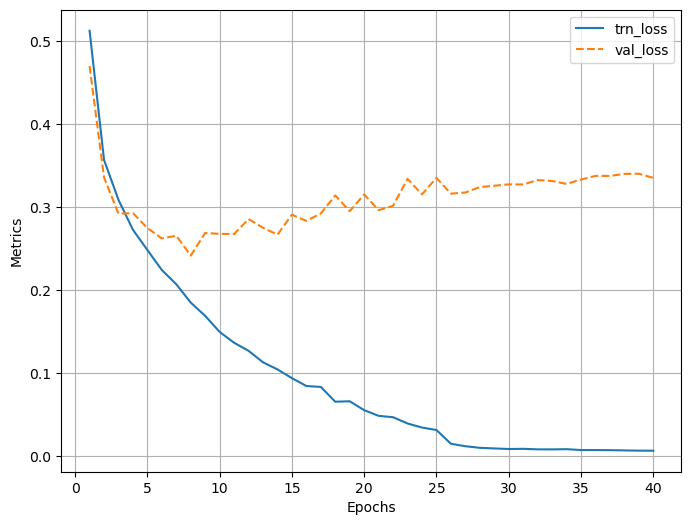
\includegraphics[width=0.6\linewidth]{first_nn/initial_train}
	\caption{Gráfico do custo de treinamento e de validação ao longo das épocas de treinamento.}
	\label{fig:note1:init_train}
\end{figure}

O exercício proposto envolve a modificação do modelo e dos processos de treinamento de forma a solucionar o problema encontrado, mas sem causar \textit{overfitting}.

\subsection{Solução do Exercício Proposto}

Diferentes abordagens para reduzir o fenômeno de \textit{underfitting} podem ser aplicadas, entre elas o aumento da taxa de aprendizado ou o aumento de épocas, aumentar a complexidade da rede neural, aumentando a quantidade de camadas escondidas, por exemplo, entre outras possibilidades. Outra possibilidade seria a redução da probabilidade associada à operação de \textit{dropout}, que poderia estar exagerada, prejudicando a rede -- apesar de que o valor de 0,25 não é considerado elevado, então é improvável que isso seja um problema.